% id: 122-34
% book: 쎈B 미적분1 · 09 정적분의 활용
% section: 유형 06 두 도형의 넓이가 같을 조건
% figure: tikz:fig-122-34
% answer: 
% answer_source: 
% variant_level: 0 (원본 전사)
% 이 파일은 build.mjs 가 items.json 에서 만든다. 고칠 때는 items.json 을 고친다.
\smash{\raisebox{1.5mm}{\dmkichul{쎈B 미적분1 122쪽 34번}}}
\noindent\begin{minipage}[t]{0.58\linewidth}\vspace{0pt}\raggedright 오른쪽 그림과 같이 $x\ge 0$에서 곡선 $y=x^3-6x+k$와 $x$축 및 $y$축으로 둘러싸인 도형의 넓이를 $S_1$, 이 곡선과 $x$축으로 둘러싸인 도형의 넓이를 $S_2$라 하자. $S_1=S_2$일 때, 상수 $k$의 값을 구하시오. \dmcondfill{$k>0$}{}\end{minipage}\hfill\begin{minipage}[t]{0.4\linewidth}\vspace{0pt}\centering \resizebox{\ifdim\width>\linewidth\linewidth\else\width\fi}{!}{% 122-34(122쪽) — 곡선 y=x^3-6x+k (k>0) 와 x축·y축이 x>=0 에서 둘러싸는 S_1, 이 곡선과 x축이 둘러싸는 S_2. 스캔 화질이 낮아 TikZ 로 다시 그림.
% 라벨은 원문 그대로 y·x·O·S_1·S_2·y=x^3-6x+k 와 원문의 지시선만. y절편의 높이는 원문처럼 개략 위치라 k 값을 그림에서 잴 수 없다.
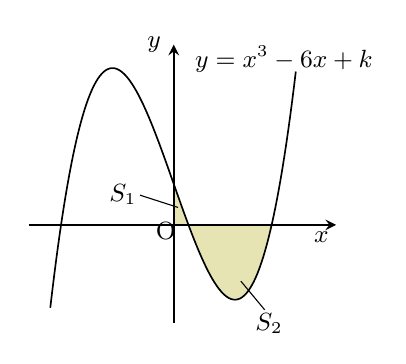
\begin{tikzpicture}[xscale=0.55, yscale=0.26, line width=0.5pt]
  \fill[olive!22] (0,0) -- plot[domain=0:0.3399, samples=30] (\x, {\x*\x*\x-6*\x+2}) -- cycle;
  \fill[olive!22] plot[domain=0.3399:2.2618, samples=50] (\x, {\x*\x*\x-6*\x+2}) -- cycle;
  \draw[->, >=stealth, line width=0.7pt] (-3.35,0) -- (3.75,0) node[below left=-1pt, font=\small] {$x$};
  \draw[->, >=stealth, line width=0.7pt] (0,-4.8) -- (0,8.8) node[left=1pt, font=\small] {$y$};
  \draw[line width=0.6pt, domain=-2.85:2.82, samples=130] plot (\x, {\x*\x*\x-6*\x+2});
  \node[below left=-2pt, font=\small, inner sep=1pt] at (0,0) {$\mathrm{O}$};
  \draw[line width=0.4pt] (-0.78,1.45) -- (0.1,0.85);
  \node[left, font=\small, inner sep=1pt] at (-0.78,1.5) {$S_1$};
  \draw[line width=0.4pt] (2.1,-4.15) -- (1.55,-2.75);
  \node[below, font=\small, inner sep=1pt] at (2.2,-4.15) {$S_2$};
  \node[right, font=\small, inner sep=2pt] at (0.35,8.1) {$y=x^3-6x+k$};
\end{tikzpicture}
}\end{minipage}\par
